% \documentclass{beamer}
% \usetheme{Szeged}

% \begin{document}

%-------------------------------------------------------------------------------
%							FITH SECTION
%-------------------------------------------------------------------------------


\section{Conclusion}
% Conclusion

\subsection{Sur l'apprentissage}

\begin{frame}
    \large
    \centering
    Conclusion sur l'apprentissage
\end{frame}

\begin{frame}
    \frametitle{Bilan de l'apprentissage}
    Par ordre croissant de réussite :
    \pause
    \begin{enumerate}[<+>]
        \item \textbf{Régression 1D} : Permet de détecter la hauteur du créneau %sur la densité d'un domaine 1D (avec la meilleure corrélation de tous les apprentissages). Elle n'a cependant pas été capable de détecter la position du créneau, probablement dû au caractère mal posé du problème inverse. DANS LE MILIU MEDICAL, LA HAUTEUR SEUL NE SUFFIT PAS
        \item \textbf{Classification 2D} : Permet de localiser l'ordonnée du créneau %en le situant par rapport aux sources sur la gauche d'un domaine 2D. En augmentant leur nombre et en plaçant certaines sources en haut (ou en bas) du domaine, on pourrait localiser avec plus de finesse l'abscisse et l'ordonnée du créneau.
        \item \textbf{Régression 2D} : Permet de prédire tous les attributs essentiels du créneau (abscisse, ordonnée, et hauteur)%, tout ceci avec une très forte précision (score personnalisé s'élevant à 93 \%). 
      \end{enumerate}
\end{frame}

\begin{frame}
    \frametitle{Absence de régularisation}
    \begin{figure}
        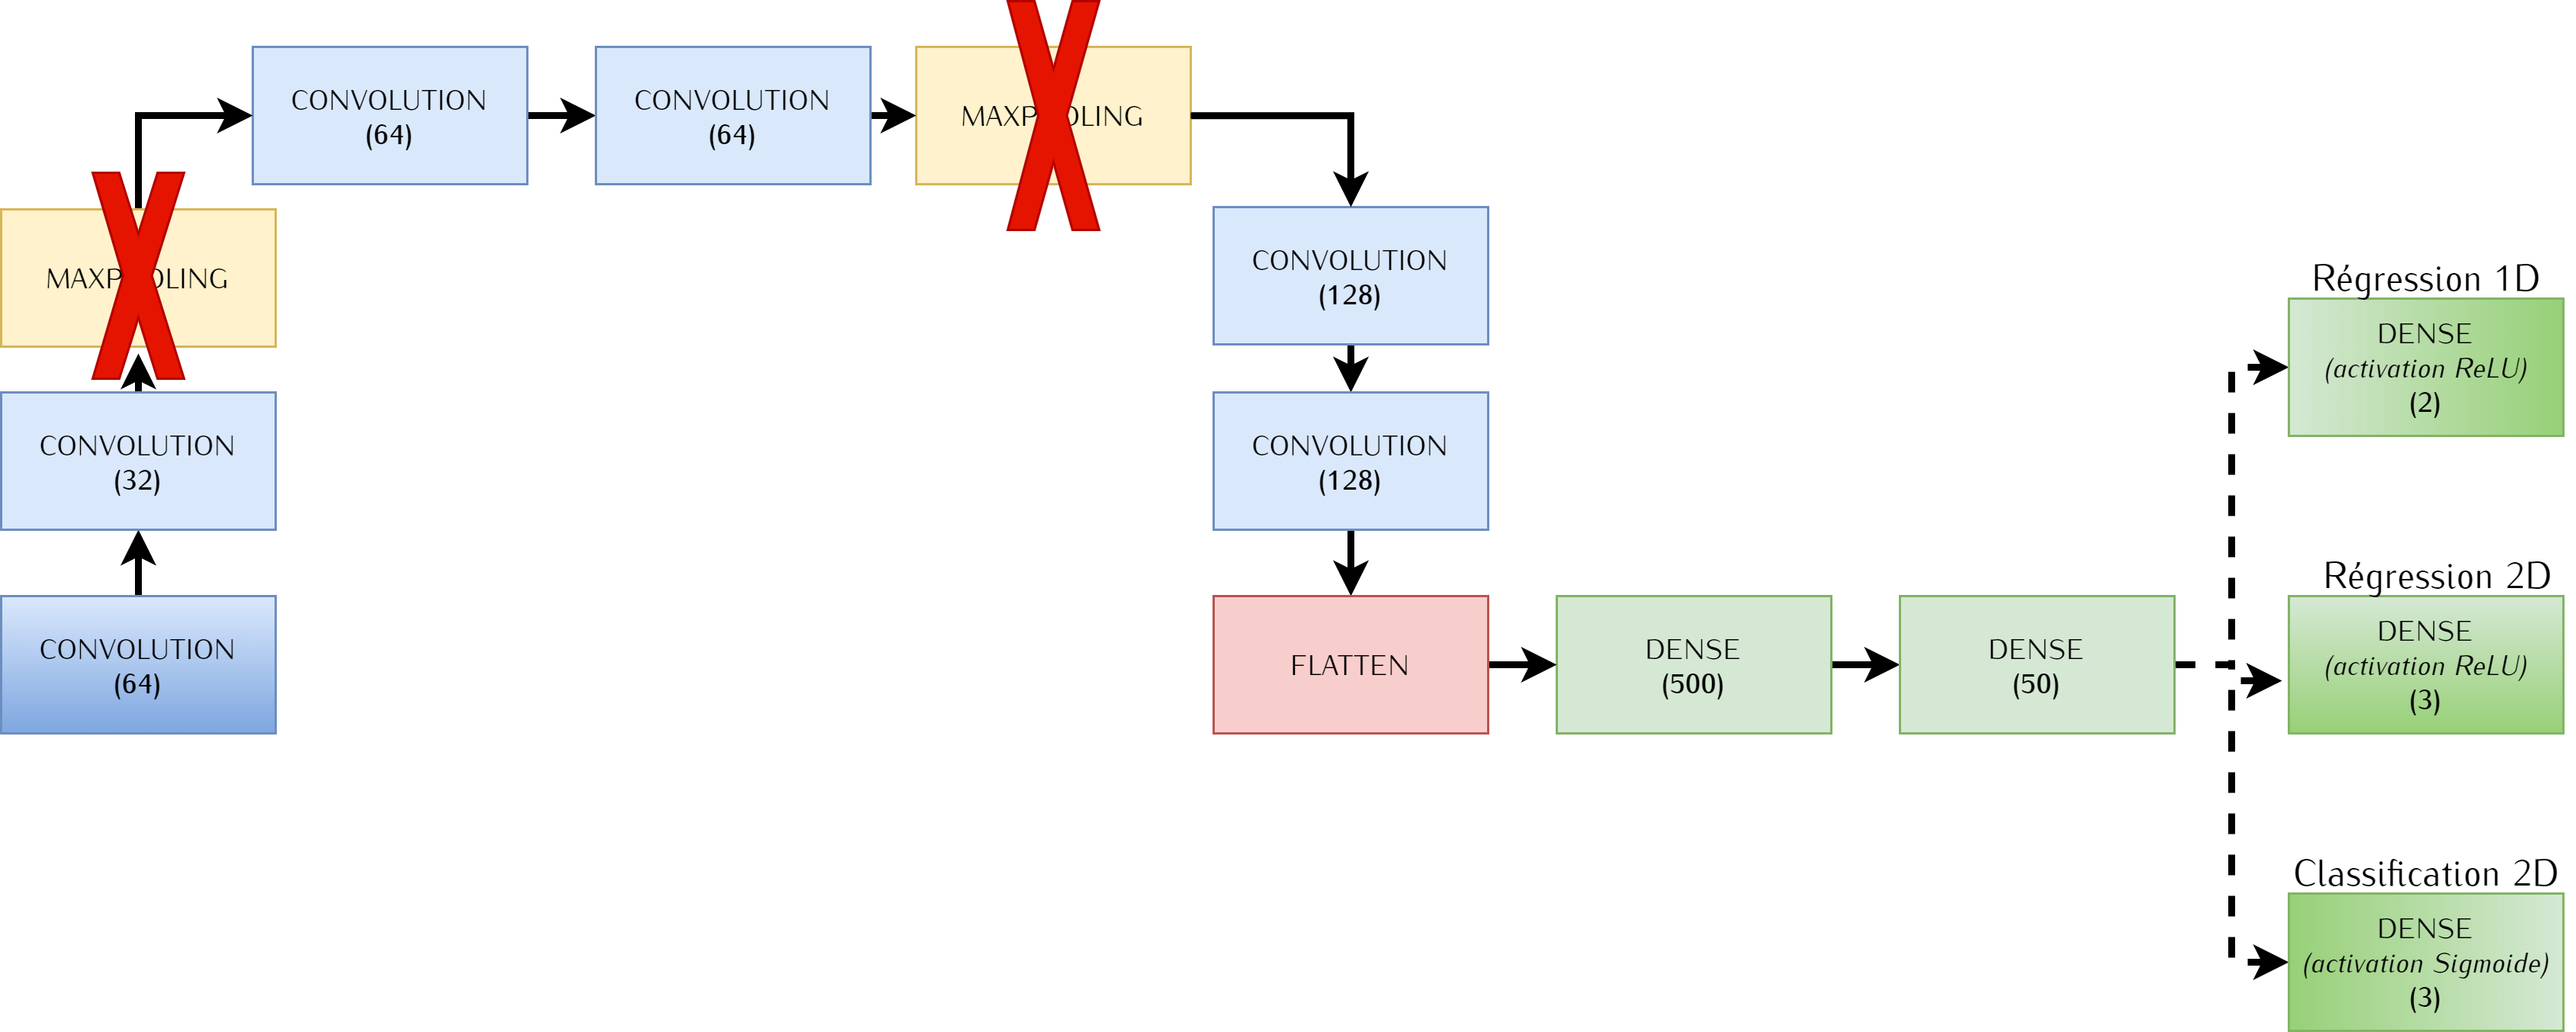
\includegraphics[width=10cm]{DRNN2MAX}       
        \caption{Architecture originale proposée par M.Vigon}
    \end{figure}
\end{frame}

\subsection{Sur le stage}

\begin{frame}
    \large
    \centering
    Conclusion sur le stage
\end{frame}

\begin{frame}
    \frametitle{Déroulement du stage}
    \begin{figure}
        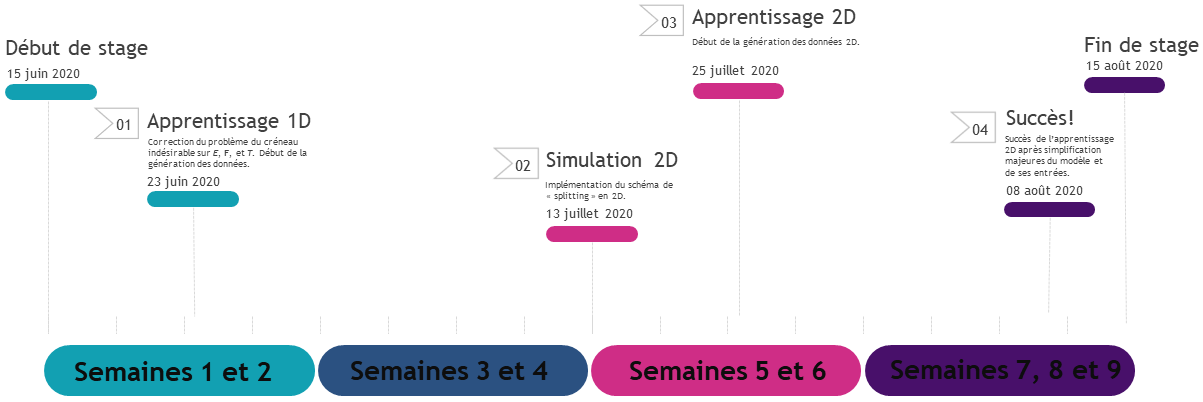
\includegraphics[width=10cm]{MilestonesRoadmap}       
        \caption{Points tournants du stage}
    \end{figure}
\end{frame}

\begin{frame}
    \frametitle{Apports et enseignements}
    \begin{itemize}[<+>]
        \item Développement C++ et Python   % Mettre en pratique les connaissances de CSMI
        \item Équations aux dérivées partielles % technique de verification
        \item Réseaux de neurones % (Keras, Tensorflow, learning rate)
        \item Expérience dans un milieu de recherche % J'ai apprecieer travailler sur IA+EDP
        % \item Point negatif: Manque de coordination (A cause du COVID). Merci encore aux profs
    \end{itemize}
\end{frame}

\begin{frame}
    \frametitle{Perspectives}
    \begin{itemize}
        \item<1-> Amélioration des résultats 
        \begin{itemize}
            \item<1-> différentes formes d'obstacles
            \item<2-> plusieurs obstacles
            \item<3-> autres formes d'opacités
        \end{itemize} 
        \item<4-> Déploiement d'un tomographe en milieu médical
        \item<5> Stage, thèse ultérieures ...
    \end{itemize}
\end{frame}

% \end{document}
